\documentclass[10pt,a4paper]{article}
\usepackage[T1]{fontenc}
\usepackage[scaled]{helvet}
\usepackage{cite}
\usepackage{url}
\usepackage{graphicx}
\usepackage{listings}
\usepackage{float}
\usepackage{amsmath}
\usepackage{listings}
\usepackage{color}
 
\definecolor{dkgreen}{rgb}{0,0.6,0}
\definecolor{gray}{rgb}{0.5,0.5,0.5}
\definecolor{mauve}{rgb}{0.58,0,0.82}
\lstset{ %
  language=Octave,                % the language of the code
  basicstyle=\footnotesize,           % the size of the fonts that are used for the code
  numbers=left,                   % where to put the line-numbers
  numberstyle=\tiny\color{gray},  % the style that is used for the line-numbers
  stepnumber=1,                   % the step between two line-numbers. If it's 1, each line 
                                  % will be numbered
  numbersep=5pt,                  % how far the line-numbers are from the code
  backgroundcolor=\color{white},      % choose the background color. You must add \usepackage{color}
  showspaces=false,               % show spaces adding particular underscores
  showstringspaces=true,         % underline spaces within strings
  showtabs=false,                 % show tabs within strings adding particular underscores
  frame=none,                   % adds a frame around the code
  rulecolor=\color{black},        % if not set, the frame-color may be changed on line-breaks within not-black text (e.g. commens (green here))
  tabsize=2,                      % sets default tabsize to 2 spaces
  breaklines=true,                % sets automatic line breaking
  breakatwhitespace=false,        % sets if automatic breaks should only happen at whitespace
  keywordstyle=\color{blue},          % keyword style
  commentstyle=\color{dkgreen},       % comment style
  stringstyle=\color{mauve},         % string literal style
  escapeinside={\%*}{*)},            % if you want to add LaTeX within your code
  morekeywords={*,...}               % if you want to add more keywords to the set
}
\usepackage{amssymb}
\usepackage{fancyhdr}
\usepackage{lastpage}
\floatstyle{boxed} 
\restylefloat{figure}
\renewcommand*\familydefault{\sfdefault}
\title{Management of Main Memory}
\author{David Lynch - david.lynch@raglansoftware.com }
\begin{document}
\maketitle
The final topics in the Operating Systems section of this course deals with the management of main memory. Once you are comfortable with creating processes, understanding how processes communicate with each other and taking advantage of threads the next concern lies with understanding these concepts. How the operating system manages main memory is a very important topic. As a programmer this will become clear if as soon as you start writing any non-trivial applications, particularly in the enterprise space. How the operating system manages memory allocated to your process has an effect on everything from how your program functions to the performance of your application. 
\end{abstract}
\section{Main Memory}
Processes are assigned an address space defined by a {\bf base register} and a {\bf limit register}. Hardware and the operating system provide protections around user processes accessing the addresses of other processes or any locations in kernel memory. However, operations that execute in Kernel mode may have access to the full address space. 
\newline\newline
A process can be located anywhere in memory, and its starting location, together with other significant locations are bound to re-locatable addresses. This address in turn is part of a mapping between {\bf logical} and {\bf physical} address locations. Binding to address locations can happen at {\bf compile time}, {\bf load time} and {\bf execution time}. In the first instance, address locations are pre-compiled to pre-determined locations in memory. With load time binding, the program can be re-located across the address space. During execution time a process may, for example, be moved from one segment in memory to another. This is determined by various characteristics of the application at runtime. 
\subsection{Logical vs. Physical Address Space}
Addresses generated by the CPU are referred to as {\bf logical addresses}. The address seen by the MMU, and stored in the {\bf memory address register} or MAR is referred to as the {\bf physical address}. The set of all logical addresses generated by a program is called it's {\bf virtual address space}. Conversely, the {\bf physical address space} is the set of all the physical addresses associated with the processes. The MMU is responsible for the mapping that exists between the two views. 
\subsection{Dynamic Loading}
So far we have required the entire process to exist in physical memory for it to be executable. Dynamic loading allows a routine to be left on secondary storage until it is required. This can be more memory-space efficient, but can have performance ramifications. For this to work, routines are kept on disk in a relocatable format. Before another routine is called the running routine may check if the new routine is already loaded. A loader then loads the routine into memory, adjusting the address space before handing control back to the program. No special operating systems intervention is required for this functionality. 
\subsection{Dynamic Linking and Shared Libraries}
Libraries that are not dynamically linked by a program are termed statically linked. Each process keeps its own copy of a statically linked library in memory. Dynamically linked libraries exist initially only as {\bf stubs} in memory. This stub contains contains instructions on how to link the library to the program. One of two courses of action are possible when a dynamically linked library is required. In the case where library has not been loaded from disk, it is loaded into memory. Otherwise, the stub will replace itself with a pointer to the address to which the dynamically linked library has been stored to memory. In this manner, multiple programs that use the same libraries will reference one copy of the code in memory. Dynamic Linking requires help from the OS is multiple processes are required to access the same address. 
\subsection{Swapping}
Processes must be in main memory to be executed, but at various points may be swapped from memory to the backing store. For example, when a process is suspended, the memory manager may move the non longer executing process from main memory to disk. Processes may be swapped back into a different address space at some point after they are swapped out. The CPU calls the {\bf dispatcher} which checks to see if the next process in the ready queue is in memory. If it is not in memory, the process gets loaded. During this action, other processes that are not under execution may be swapped out to free up sufficient memory for the replacement process. {\bf Context Switch} time is a pure cost in this process, and is a direct function of the size of the program being executed, the performance characteristics of the backing store and other underlying hardware. For a process to be a candidate for disk swapping it must be {\bf completely idle}. In particular, waiting on I/O or for the CPU is not a sufficient reason to swap the process to the disk. 
\subsection{Memory Allocation}
In order to manage memory, division into fixed size partitions is the simplest approach. Each of these partitions will contain exactly one process. With this strategy, the number of processes is bound by the size of the physical memory space. Each partition is known as a {\bf hole}. The process acquires and releases each hole as it is swapped in and out of memory. The operating system may merge smaller holes into bigger ones to facilitate the loading of bigger processes into memory. The problem of satisfying a request for $n$ bytes of space from a list of free memory holes is one of dynamic allocation. One approach is to allocate the first hole that is large enough. The {\best fit} approach will allocate the smallest hole that is big enough, leaving the smallest hole left over. Lastly, the worst fit approach picks the worst possible fit for the process, ensuring the largest hole remains. First fit is faster, but both best and worst fit have better, and similar memory utilization characteristics. 
\subsection{Fragmentation}
In any allocation strategy when small unusable memory segments are left over, the system is suffering from memory fragmentation. There are two flavours of fragmentation that essentially differ by whether the left over memory that is unusable is contained in an allocated block, or in free space external to a block. 
\subsubsection{External Fragmentation}
The previously discussed strategies will inevitably cause external fragmentation over the lifetime of a power-up. Swapping back and forth from disk using these strategies will cause small unusable holes of memory to appear. Statistical analysis of first fit shows that given $n$ holes of memory, another $0.5n$ holes will be lost to fragmentation. In order to combat this phenomenon, {\bf compaction} can be leveraged. This is the shuffling of free memory so that smaller blocks become one block. One approach to compaction is to move processes to lower sections of memory and holes to higher sections of memory. However, compaction is pure cost and, depending on the characteristics of the system, is an expensive operation. 
\subsubsection{Internal Fragmentation}
Generally holes of memory will not be allocated in the exact size required. The overhead on minute leftover blocks can be worse than giving free memory away. However, this has the effect of leaving memory allocated to the process that is not actually used by that process, nor is it usable by any other process. 
\section{Paging}
Paging is a memory management scheme that allows the physical address space of a process to be non-contiguous. This avoids the problem of fitting memory chunks of various sizes into contiguous main memory. This is typically implemented in hardware with very low level OS support. Physical memory is broken into fixed sizes known as {\bf frames}. Logical memory is broken into blocks of the same size known as {\bf pages}. When a process is executing its pages are loaded into available frames. Every CPU generated address is divided into {\bf page number} and {\bf page offset}. The page number is an index into the {\bf page table}, which holds the direct logical-to-physical mapping. It contains the base address of each page and the address of the corresponding frame in physical memory. The size of the page is fixed and defined by the hardware, but can range from 512-bytes to 16 megabytes. 
\newline\newline
If the logical address size is $2^m$ and the page size is $2^m$ addressing units then the higher order $m-n$ bits are the page number $p$ and the lower order $n$ bits are the {\bf page offset} or {\bf displacement} denoted as $d$. Figures \ref{paging}} and \ref{page mapping} show both the general configuration and an example mapping. 
\begin{figure}
\caption{The basics of paging.\cite{OSCONCEPTS}}
\begin{center}
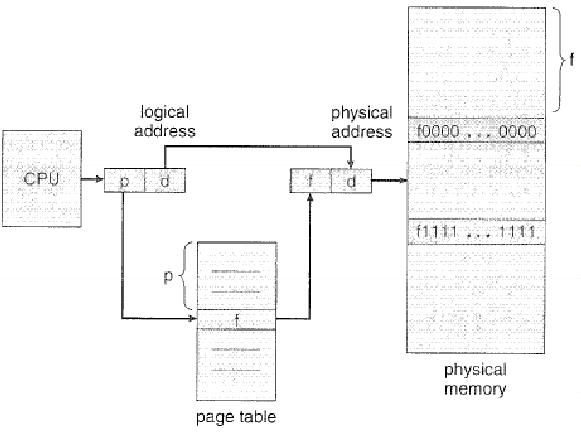
\includegraphics[scale=0.45]{../images/paging.png}
\label{paging}
\end{center}
\end{figure}
\begin{figure}
\caption{A before and after view of an example page mapping. \cite{OSCONCEPTS}}
\begin{center}
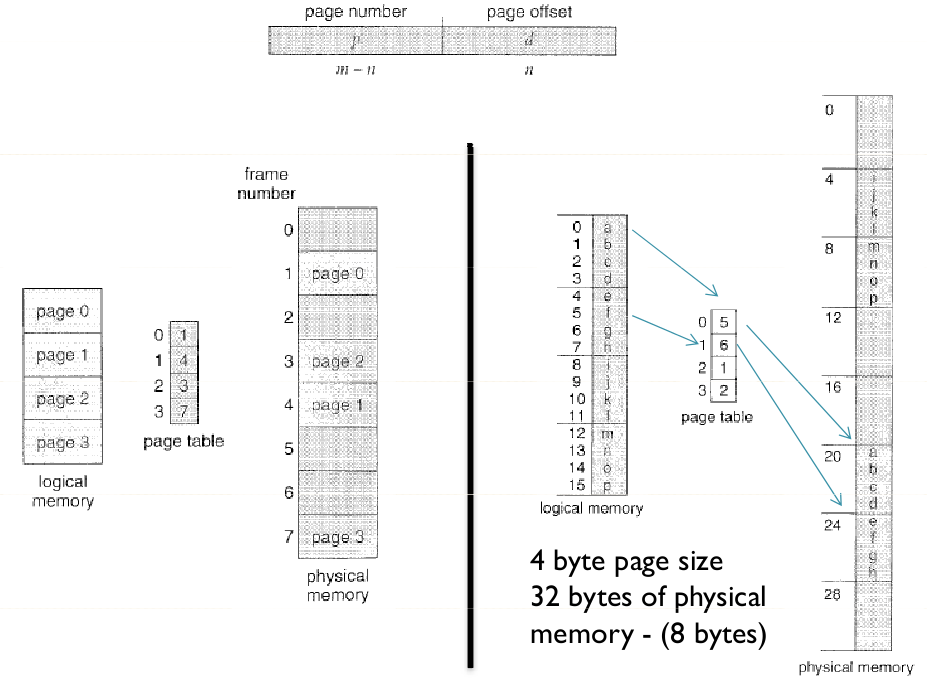
\includegraphics[scale=0.45]{../images/page-mapping.png}
\label{page mapping}
\end{center}
\end{figure}
Since any free frame can be allocated to a process that needs it, there is no external fragmentation. However, since frames are allocated in units, any time a process does not coincide with a page boundary we get internal fragmentation. For example, given a page-size of 2048 bytes, a process of size 72,766 bytes needs 35 full pages plus 1086 bytes left over. Therefore 36 pages are allocated and 962 bytes are lost to internal fragmentation. The statistical average expense is one have page of internal fragmentation per process. 
\newline\newline
A {\bf frame table} is managed by the OS which details frame availability and allocation. Each entry contains the state of the frame and to which page the frame is mapped. The OS will also manage one {\bf page table} per process, meaning paging will add to context switch overhead. 


\bibliography{../biblio/techfundamentals.bib}{}
\bibliographystyle{plain}
\begin{center}
{\small \copyright  David Lynch 2012. Do not reproduce without written permission.}
\end{center}
\end{document}
